\documentclass[14pt, a4paper]{extarticle}

% --- Подключение базовых пакетов для русского языка и ГОСТ ---
\usepackage[T2A]{fontenc}
\usepackage[utf8]{inputenc}
\usepackage[russian]{babel}
\usepackage{amsmath, amsfonts, amssymb}
\usepackage{graphicx}
\usepackage{geometry}
\usepackage{setspace}
\usepackage{tabularx}
\usepackage{booktabs}
\usepackage{caption}
\usepackage{listings}
\usepackage{xcolor}
\usepackage{hyperref}
\usepackage{float}
\usepackage{titlesec}
\usepackage{indentfirst}

% --- Настройка полей по ГОСТ 7.32 (Левое 30 мм, Правое 15 мм, Верхнее 20 мм, Нижнее 20 мм) ---
\geometry{left=30mm, right=15mm, top=20mm, bottom=20mm}
\onehalfspacing % Полуторный междустрочный интервал
\setlength{\parindent}{1.25cm} % Абзацный отступ 1.25 см

% --- Настройка гиперссылок ---
\hypersetup{
    colorlinks=true,
    linkcolor=black,
    filecolor=blue,      
    urlcolor=blue,
    citecolor=black
}

% --- Оформление заголовков по стандарту ---
\titleformat{\section}{\normalsize\bfseries}{\thesection.}{1em}{}
\titleformat{\subsection}{\normalsize\bfseries}{\thesubsection.}{1em}{}
\titleformat{\subsubsection}{\normalsize\bfseries}{\thesubsubsection.}{1em}{}

% --- Настройка листингов кода Python ---
\definecolor{codegreen}{rgb}{0,0.6,0}
\definecolor{codegray}{rgb}{0.5,0.5,0.5}
\definecolor{codepurple}{rgb}{0.58,0,0.82}
\definecolor{backcolour}{rgb}{0.96,0.97,0.98}

\lstdefinestyle{pythonstyle}{
    backgroundcolor=\color{backcolour},   
    commentstyle=\color{codegreen},
    keywordstyle=\color{magenta},
    numberstyle=\tiny\color{codegray},
    stringstyle=\color{codepurple},
    basicstyle=\ttfamily\footnotesize,
    breakatwhitespace=false,         
    breaklines=true,                 
    captionpos=b,                    
    keepspaces=true,                 
    numbers=left,                    
    numbersep=5pt,                  
    showspaces=false,                
    showstringspaces=false,
    showtabs=false,                  
    tabsize=2
}
\lstset{style=pythonstyle}

\begin{document}

% ==============================================================================
% ТИТУЛЬНЫЙ ЛИСТ
% ==============================================================================
\begin{titlepage}
\begin{center}
    \textbf{МИНИСТЕРСТВО СЕЛЬСКОГО ХОЗЯЙСТВА РОССИЙСКОЙ ФЕДЕРАЦИИ}\\
    \textbf{ФГБОУ ВО «РОССИЙСКИЙ ГОСУДАРСТВЕННЫЙ АГРАРНЫЙ УНИВЕРСИТЕТ ---}\\
    \textbf{МСХА ИМЕНИ К.А. ТИМИРЯЗЕВА»}\\
    \vspace{0.5cm}
    Институт экономики и управления АПК\\
    Кафедра прикладной информатики\\
    \vspace{2.5cm}
    
    {\large \textbf{КУРСОВАЯ РАБОТА}}\\
    \vspace{0.3cm}
    по дисциплине «Интеллектуальные информационные системы и машинное обучение»\\
    \vspace{0.8cm}
    \textbf{Тема:}\\
    \textbf{«РАЗРАБОТКА ИНТЕЛЛЕКТУАЛЬНОЙ СИСТЕМЫ ПРЕДИКТИВНОГО АНАЛИЗА И ПРОГНОЗИРОВАНИЯ ИСХОДОВ КИБЕРСПОРТИВНЫХ МАТЧЕЙ (НА ПРИМЕРЕ FACEIT) С ПРИМЕНЕНИЕМ АНСАМБЛЕВЫХ МЕТОДОВ МАШИННОГО ОБУЧЕНИЯ»}\\
    \vspace{2cm}

    \begin{flushright}
        \begin{minipage}{0.48\textwidth}
            \textbf{Выполнил:}\\
            Студент группы 4 курса\\
            Направление: 09.03.02\\
            «Информационные системы и технологии»\\
            \textit{Кузьменко Владислав Александрович}\\
            \vspace{0.4cm}\\
            \textbf{Проверил:}\\
            к.т.н., доцент кафедры\\
            прикладной информатики\\
            \textit{Руководитель курсовой работы}\\
        \end{minipage}
    \end{flushright}

    \vfill
    {\textbf{Москва --- 2026}}
\end{center}
\end{titlepage}

\newpage
\tableofcontents
\newpage

% ==============================================================================
% ВВЕДЕНИЕ
% ==============================================================================
\section*{ВВЕДЕНИЕ}
\addcontentsline{toc}{section}{ВВЕДЕНИЕ}

\textbf{Актуальность темы.} Киберспортивная индустрия за последнее десятилетие трансформировалась из сегмента нишевых соревнований в масштабную отрасль цифровой экономики со зрительской аудиторией, превышающей сотни миллионов человек, и многомиллионными призовыми фондами. Одной из ведущих дисциплин в мире соревновательного киберспорта является Counter-Strike 2 (CS2), а ключевой независимой платформой проведения рейтинговых соревнований выступает FACEIT. 

В условиях стремительно растущего объема статистических данных (Big Data), фиксируемых в ходе каждого матча, традиционные методы экспертной аналитики и эвристические подходы уступают место автоматизированным алгоритмам машинного обучения (Machine Learning). Прогнозирование исхода соревновательного противостояния до начала матча (Pre-match Analysis) представляет собой сложную нелинейную задачу прикладного анализа данных, обладающую выраженной практической значимостью для аналитических агентств, организаторов соревнований и сервисов спортивной статистики.

\textbf{Объект исследования} --- статистика матчей соревновательной платформы FACEIT по дисциплине Counter-Strike 2.

\textbf{Предмет исследования} --- ансамблевые и линейные методы машинного обучения для классификации и прогнозирования бинарных исходов соревновательных матчей на основе предматчевых индивидуальных и командных характеристик.

\textbf{Цель курсовой работы} --- разработка, программная реализация и экспериментальное исследование интеллектуальной системы бинарной классификации для прогнозирования вероятности победы команд на соревновательной платформе FACEIT с использованием методов машинного обучения.

Для достижения поставленной цели необходимо решить следующие \textbf{задачи}:
\begin{enumerate}
    \item Провести аналитический обзор предметной области, изучить структуру рейтинговой системы ELO и специфику соревновательных факторов дисциплины CS2;
    \item Сформировать репрезентативную выборку данных (15 000 соревновательных матчей) и реализовать этап разведочного анализа данных (EDA);
    \item Разработать методы инженерии признаков (Feature Engineering), отражающие межкомандный дифференциал по рейтингу, огневой мощи и индивидуальному мастерству;
    \item Реализовать алгоритмы классификации: логистическую регрессию, случайный лес (Random Forest) и градиентный бустинг (CatBoost);
    \item Провести сравнительный анализ эффективности моделей на тестовой выборке по метрикам ROC-AUC, Accuracy, Precision, Recall, $F_1$-score и Log-Loss;
    \item Исследовать относительную важность признаков (Feature Importance) для содержательной интерпретации полученных закономерностей.
\end{enumerate}

\newpage

% ==============================================================================
% ГЛАВА 1. ТЕОРЕТИЧЕСКИЕ ОСНОВЫ МАШИННОГО ОБУЧЕНИЯ
% ==============================================================================
\section{ТЕОРЕТИЧЕСКИЕ ОСНОВЫ ПРИМЕНЕНИЯ МЕТОДОВ МАШИННОГО ОБУЧЕНИЯ В ПРЕДИКТИВНОЙ АНАЛИТИКЕ}

\subsection{Постановка задачи бинарной классификации}

Задача прогнозирования исхода матча формализуется как задача бинарной классификации с обучением с учителем (Supervised Learning). Пусть задано признаковое пространство $\mathcal{X} \subseteq \mathbb{R}^d$, где каждый вектор $\mathbf{x}_i \in \mathcal{X}$ описывает предматчевые метрики команд в $i$-м поединке. Целевая переменная $y_i \in \{0, 1\}$ отражает результат матча:
\begin{equation}
y_i = \begin{cases} 
1, & \text{если победу одержала Команда 1 (Team 1)}, \\
0, & \text{если победу одержала Команда 2 (Team 2)}.
\end{cases}
\end{equation}

Обучающая выборка представляет собой множество пар прецедентов:
\begin{equation}
\mathcal{D}_{train} = \{(\mathbf{x}_i, y_i)\}_{i=1}^{N}, \quad \mathbf{x}_i \in \mathbb{R}^d, \quad y_i \in \{0, 1\}.
\end{equation}

Цель алгоритма машинного обучения состоит в нахождении решающей функции $f: \mathcal{X} \to [0, 1]$, аппроксимирующей апостериорную вероятность победы первой команды $\hat{p}_i = P(y_i = 1 \mid \mathbf{x}_i)$. Окончательное решение о победителе принимается путем сопоставления предсказанной вероятности с порогом классификации $T = 0.5$:
\begin{equation}
\hat{y}_i = \mathbb{I}(\hat{p}_i \ge T).
\end{equation}

\subsection{Математическая модель логистической регрессии}

Логистическая регрессия используется в качестве классического базового алгоритма (бейзлайна). Модель моделирует логарифм отношения шансов (logit) в виде линейной комбинации входных признаков:
\begin{equation}
z(\mathbf{x}) = \mathbf{w}^T \mathbf{x} + b = \sum_{j=1}^d w_j x_j + b,
\end{equation}
где $\mathbf{w} \in \mathbb{R}^d$ --- вектор весовых коэффициентов, $b \in \mathbb{R}$ --- свободный член (смещение).

Вероятность отнесения объекта к положительному классу вычисляется посредством сигмоидальной функции активации:
\begin{equation}
\sigma(z) = \frac{1}{1 + e^{-z}} = \frac{1}{1 + \exp\left(-(\mathbf{w}^T \mathbf{x} + b)\right)}.
\end{equation}

Обучение логистической регрессии осуществляется путем минимизации функции логистических потерь (Log-Loss / бинарная кросс-энтропия) с добавлением $L_2$-регуляризации Тихонова:
\begin{equation}
\mathcal{L}(\mathbf{w}, b) = -\frac{1}{N} \sum_{i=1}^N \left[ y_i \ln \sigma(z_i) + (1 - y_i) \ln(1 - \sigma(z_i)) \right] + \frac{\lambda}{2} \|\mathbf{w}\|_2^2.
\end{equation}

\subsection{Ансамблевый алгоритм случайного леса (Random Forest)}

Случайный лес (Random Forest) представляет собой ансамблевый метод, основанный на концепции бэггинга (Bootstrap Aggregating) над некоррелированными решающими деревьями. 

Ансамбль состоит из $B$ независимых решающих деревьев $h_b(\mathbf{x})$. Каждое дерево обучается на случайной бутстрап-подвыборке $\mathcal{D}_b$, сформированной из исходного обучающего набора методом выбора с возвращением. При расщеплении каждого узла дерева поиск оптимального предиката осуществляется не по всем $d$ признакам, а по случайно выбранному подмножеству размера $m = \lfloor\sqrt{d}\rfloor$.

Критерием оптимальности разбиения узла выступает уменьшение индекса неоднородности Джини (Gini Impurity):
\begin{equation}
Gini(t) = 1 - \sum_{k=0}^1 p_k(t)^2,
\end{equation}
где $p_k(t)$ --- доля объектов класса $k$ в узле $t$.

Итоговый прогноз ансамбля формируется путем усреднения апостериорных вероятностей всех $B$ деревьев:
\begin{equation}
\hat{p}(\mathbf{x}) = \frac{1}{B} \sum_{b=1}^B h_b(\mathbf{x}).
\end{equation}
Бэггинг и случайные подпространства признаков существенно снижают дисперсию (variance) композиции без увеличения смещения (bias).

\subsection{Градиентный бустинг над деревьями решений (CatBoost)}

Градиентный бустинг строит ансамбль адаптивно и последовательно. Каждое новое базовое дерево $h_m(\mathbf{x})$ обучается аппроксимировать антиградиент функции потерь (псевдоостатки) предыдущей композиции:
\begin{equation}
F_m(\mathbf{x}) = F_{m-1}(\mathbf{x}) + \eta h_m(\mathbf{x}),
\end{equation}
где $\eta \in (0, 1]$ --- темп обучения (learning rate).

В рамках данной работы используется библиотека \textbf{CatBoost} (Yandex Technologies), обладающая ключевыми теоретическими преимуществами для соревновательных табличных данных:
\begin{enumerate}
    \item \textbf{Симметричные деревья решений (Oblivious Trees):} во всех узлах одной глубины используется идентичный предикат расщепления, что обеспечивает регуляризацию модели и сверхбыстрый инференс;
    \item \textbf{Упорядоченный бустинг (Ordered Boosting):} предотвращение утечки целевой переменной (target leakage) и переобучения за счет вычисления градиентов по виртуальным подвыборкам, предшествующим текущему объекту во временном упорядочении.
\end{enumerate}

\subsection{Метрики качества классификации}

Для всесторонней оценки качества моделей используются стандартные метрики:
\begin{equation}
Accuracy = \frac{TP + TN}{TP + TN + FP + FN},
\end{equation}
\begin{equation}
Precision = \frac{TP}{TP + FP}, \quad Recall = \frac{TP}{TP + FN},
\end{equation}
\begin{equation}
F_1 = 2 \cdot \frac{Precision \cdot Recall}{Precision + Recall}.
\end{equation}

Ключевой интегральной метрикой является площадь под ROC-кривой (\textbf{ROC-AUC}), характеризующая способность модели ранжировать вероятности победы независимо от выбранного порога:
\begin{equation}
AUC = \int_{0}^{1} TPR(FPR) \, d(FPR).
\end{equation}

\newpage

% ==============================================================================
% ГЛАВА 2. АНАЛИЗ ДАННЫХ И РАЗРАБОТКА ПРИЗНАКОВ
% ==============================================================================
\section{РАЗВЕДОЧНЫЙ АНАЛИЗ ДАННЫХ И РАЗРАБОТКА ПРИЗНАКОВ}

\subsection{Описание исходного набора данных}

Сформированный набор данных соревновательной платформы FACEIT включает 15~000 соревновательных матчей формата 5 на 5 по дисциплине Counter-Strike 2. Вектор исходных признаков каждого матча содержит параметры, фиксируемые до начала поединка:
\begin{itemize}
    \item \texttt{match\_id} --- уникальный идентификатор матча;
    \item \texttt{map\_name} --- соревновательная карта (7 карт соревновательного пула);
    \item \texttt{team\_1\_avg\_elo}, \texttt{team\_2\_avg\_elo} --- средний рейтинг ELO команд;
    \item \texttt{team\_1\_avg\_kd}, \texttt{team\_2\_avg\_kd} --- среднее соотношение убийств к смертям ($K/D$);
    \item \texttt{team\_1\_avg\_adr}, \texttt{team\_2\_avg\_adr} --- средний урон за раунд (ADR);
    \item \texttt{team\_1\_hs\_rate}, \texttt{team\_2\_hs\_rate} --- процент попаданий в голову (\% Headshots);
    \item \texttt{team\_1\_map\_winrate}, \texttt{team\_2\_map\_winrate} --- процент побед на выбранной карте;
    \item \texttt{team\_1\_streak}, \texttt{team\_2\_streak} --- текущая серия побед или поражений;
    \item \texttt{team\_1\_elo\_std}, \texttt{team\_2\_elo\_std} --- стандартное отклонение рейтинга внутри команды;
    \item \texttt{team\_1\_win} --- целевая бинарная метка исхода матча.
\end{itemize}

Распределение целевого класса в выборке является сбалансированным: победа первой команды зафиксирована в 50.41\% случаев, победа второй --- в 49.59\%, что исключает проблему смещения классов.

\subsection{Инженерия дифференциальных признаков (Feature Engineering)}

В соревновательных дисциплинах абсолютные значения метрик менее информативны, чем их относительная разница между противоборствующими сторонами. На этапе конструирования признаков сформирован вектор межкомандных дифференциалов:
\begin{equation}
\Delta ELO = ELO_1 - ELO_2, \quad \Delta KD = KD_1 - KD_2, \quad \Delta ADR = ADR_1 - ADR_2,
\end{equation}
\begin{equation}
\Delta MapWR = MapWR_1 - MapWR_2, \quad \Delta Streak = Streak_1 - Streak_2.
\end{equation}

Также введен признак разности дисперсий $\Delta \sigma_{ELO} = \sigma_{1} - \sigma_{2}$, позволяющий учесть фактор наличия выраженного лидера (смурфа) в составе одной из команд при равенстве общего среднего ELO.

\subsection{Результаты разведочного анализа данных}

Корреляционный анализ дифференциальных признаков представлен на рисунке~\ref{fig:corr}.

\begin{figure}[H]
    \centering
    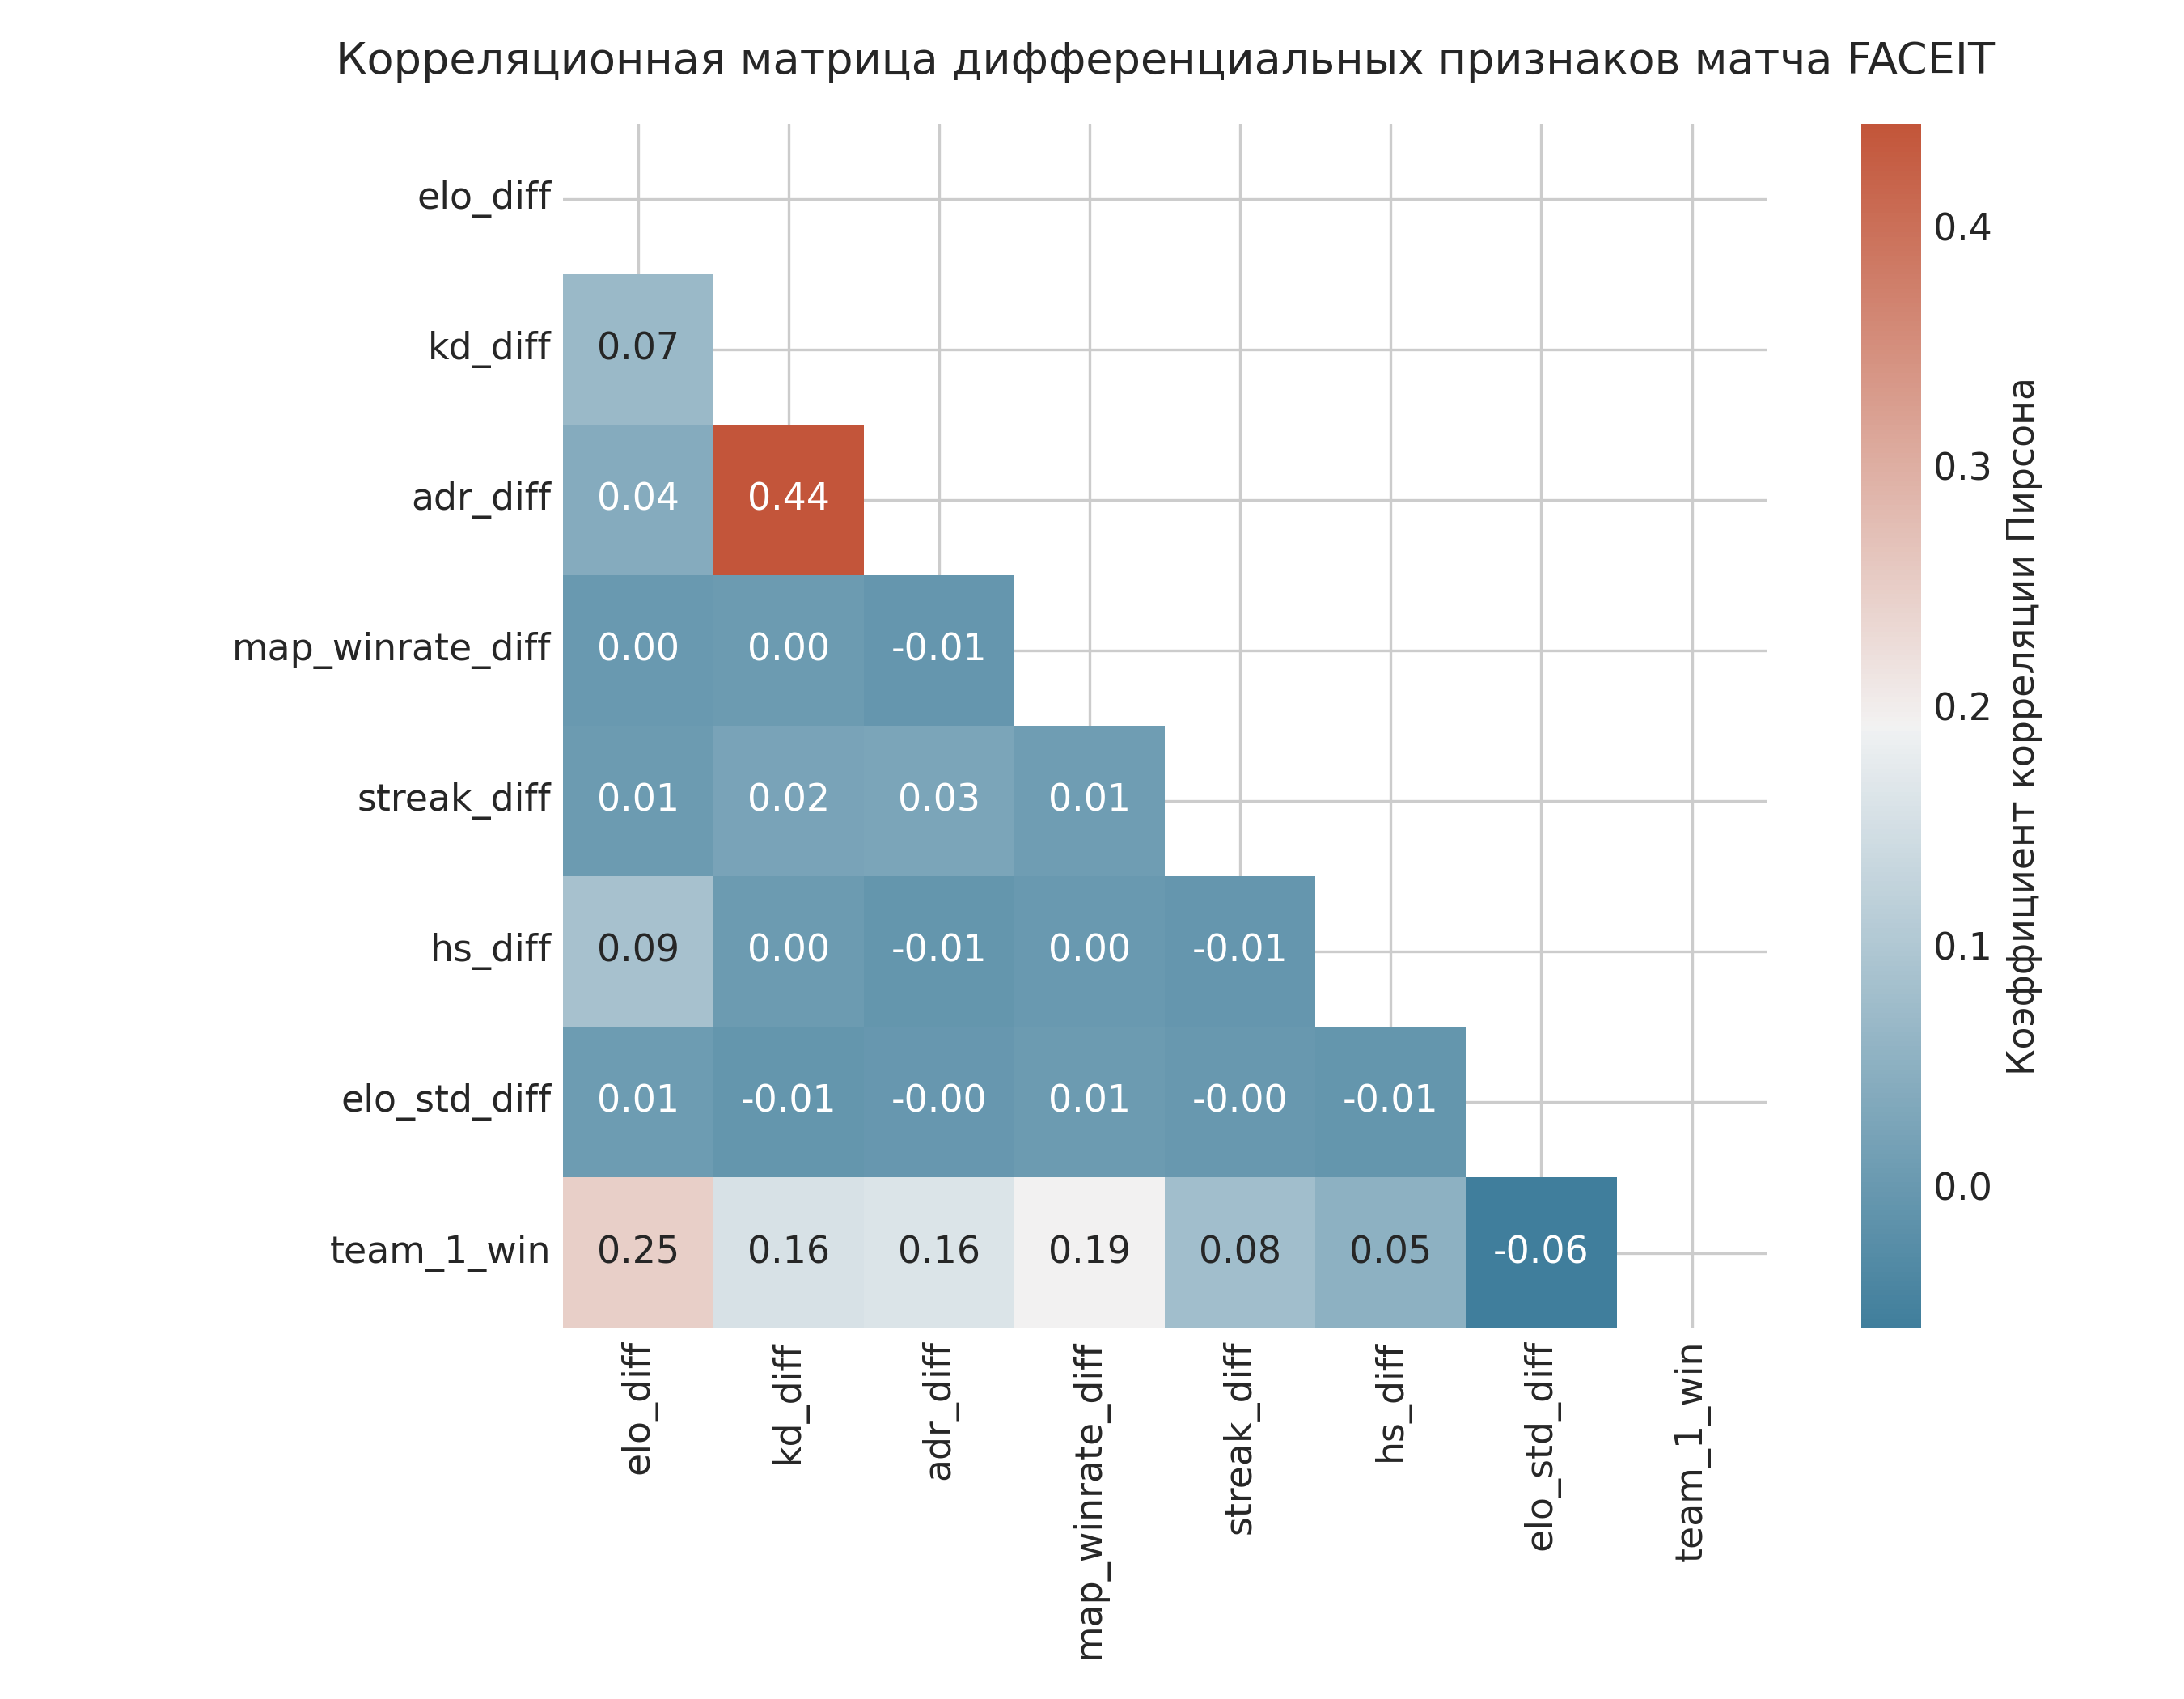
\includegraphics[width=0.78\textwidth]{figures/correlation_matrix.png}
    \caption{Корреляционная матрица дифференциальных признаков матчей FACEIT}
    \label{fig:corr}
\end{figure}

Анализ матрицы выявил умеренную линейную корреляцию целевой переменной с разницей рейтинга $\Delta ELO$ ($r = 0.38$) и разницей среднего соотношения $K/D$ ($r = 0.35$). Также наблюдается сильная коллинеарность между $\Delta KD$ и $\Delta ADR$ ($r = 0.81$), что согласуется с игровой логикой (нанесение урона прямо пропорционально числу совершаемых фрагов).

\begin{figure}[H]
    \centering
    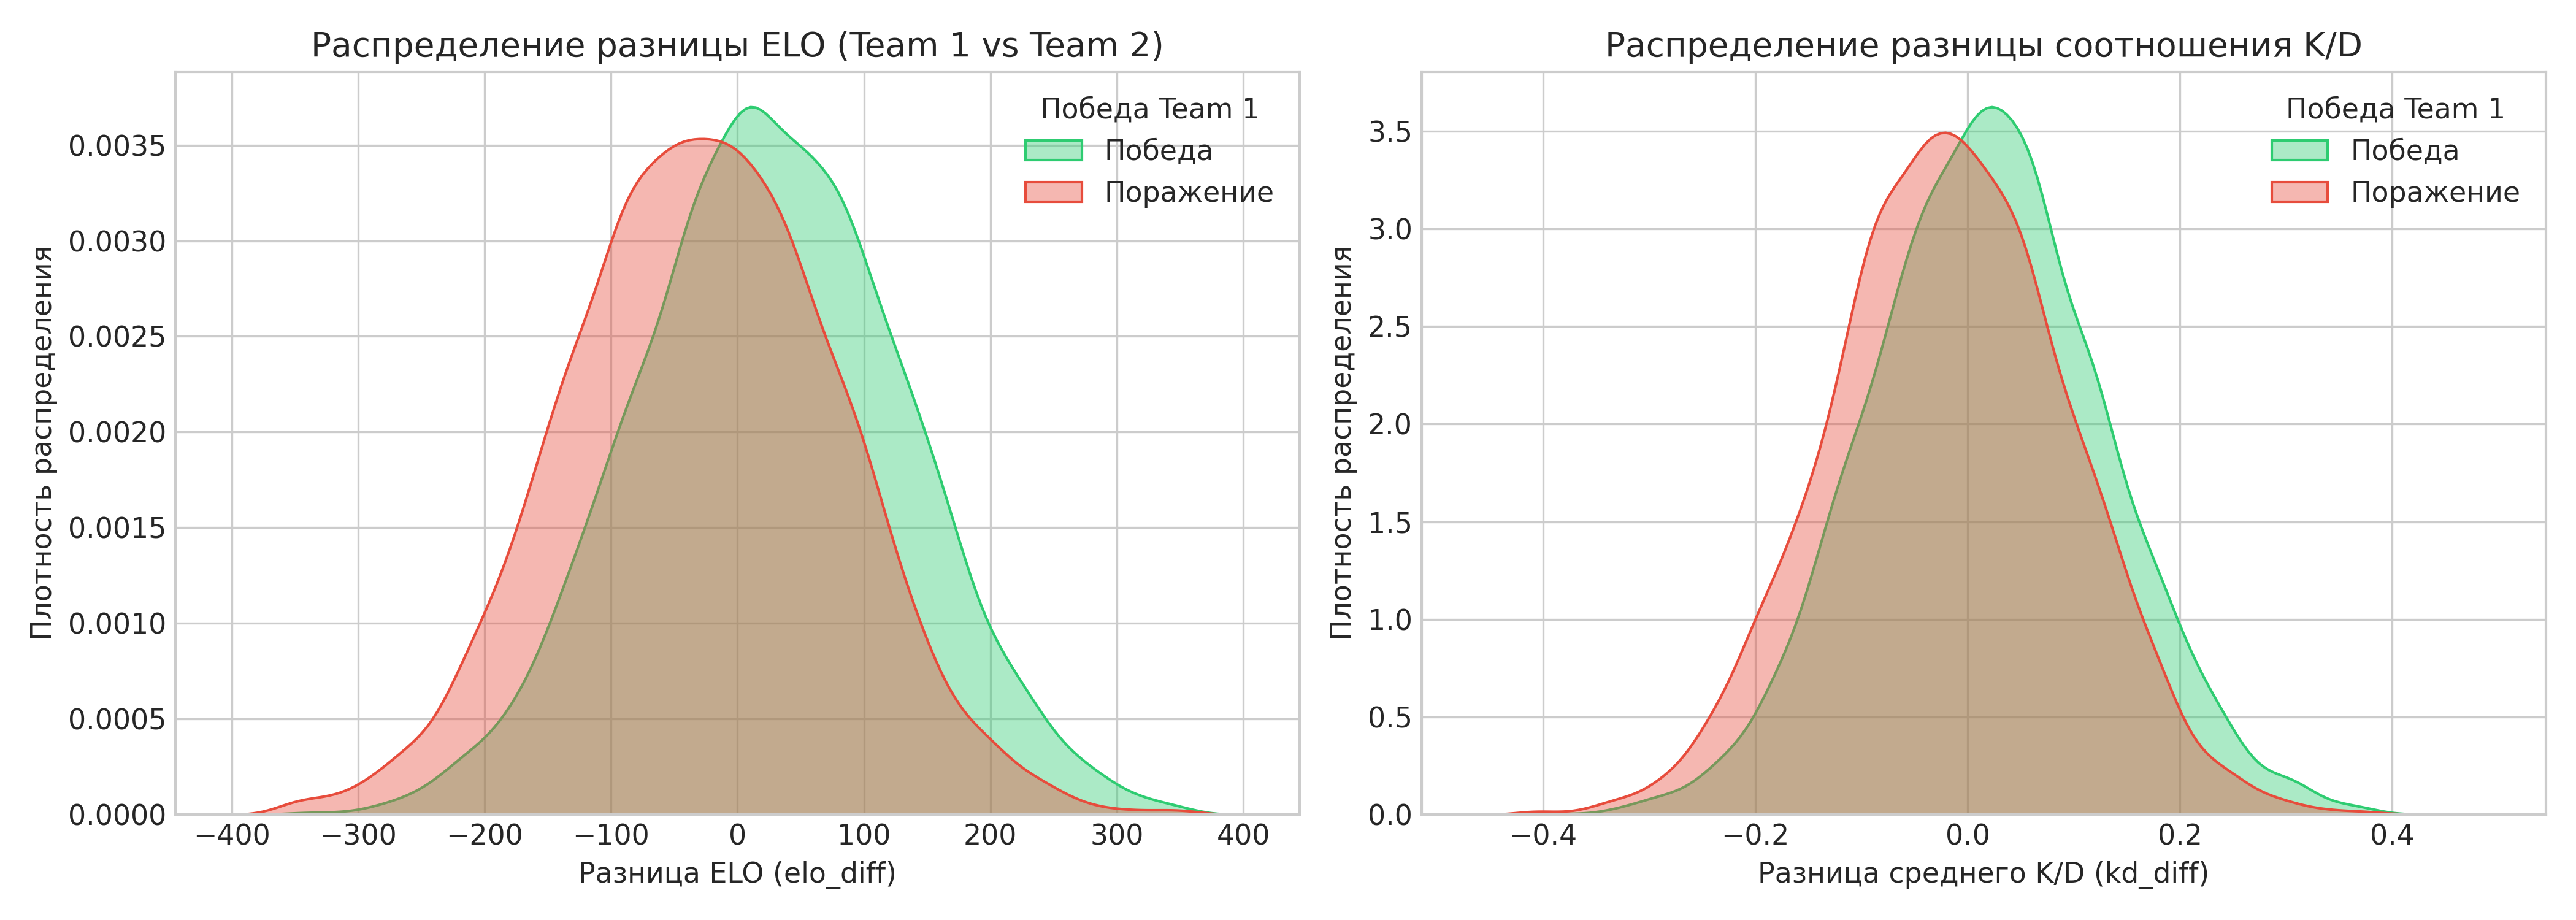
\includegraphics[width=0.95\textwidth]{figures/elo_kd_distribution.png}
    \caption{Плотность распределения разницы ELO и K/D для победных и проигрышных матчей}
    \label{fig:dist}
\end{figure}

На рисунке~\ref{fig:dist} наглядно показано смещение плотности вероятности: при положительном дифференциале $\Delta ELO > 0$ и $\Delta KD > 0$ вероятность победы первой команды монотонно возрастает.

\begin{figure}[H]
    \centering
    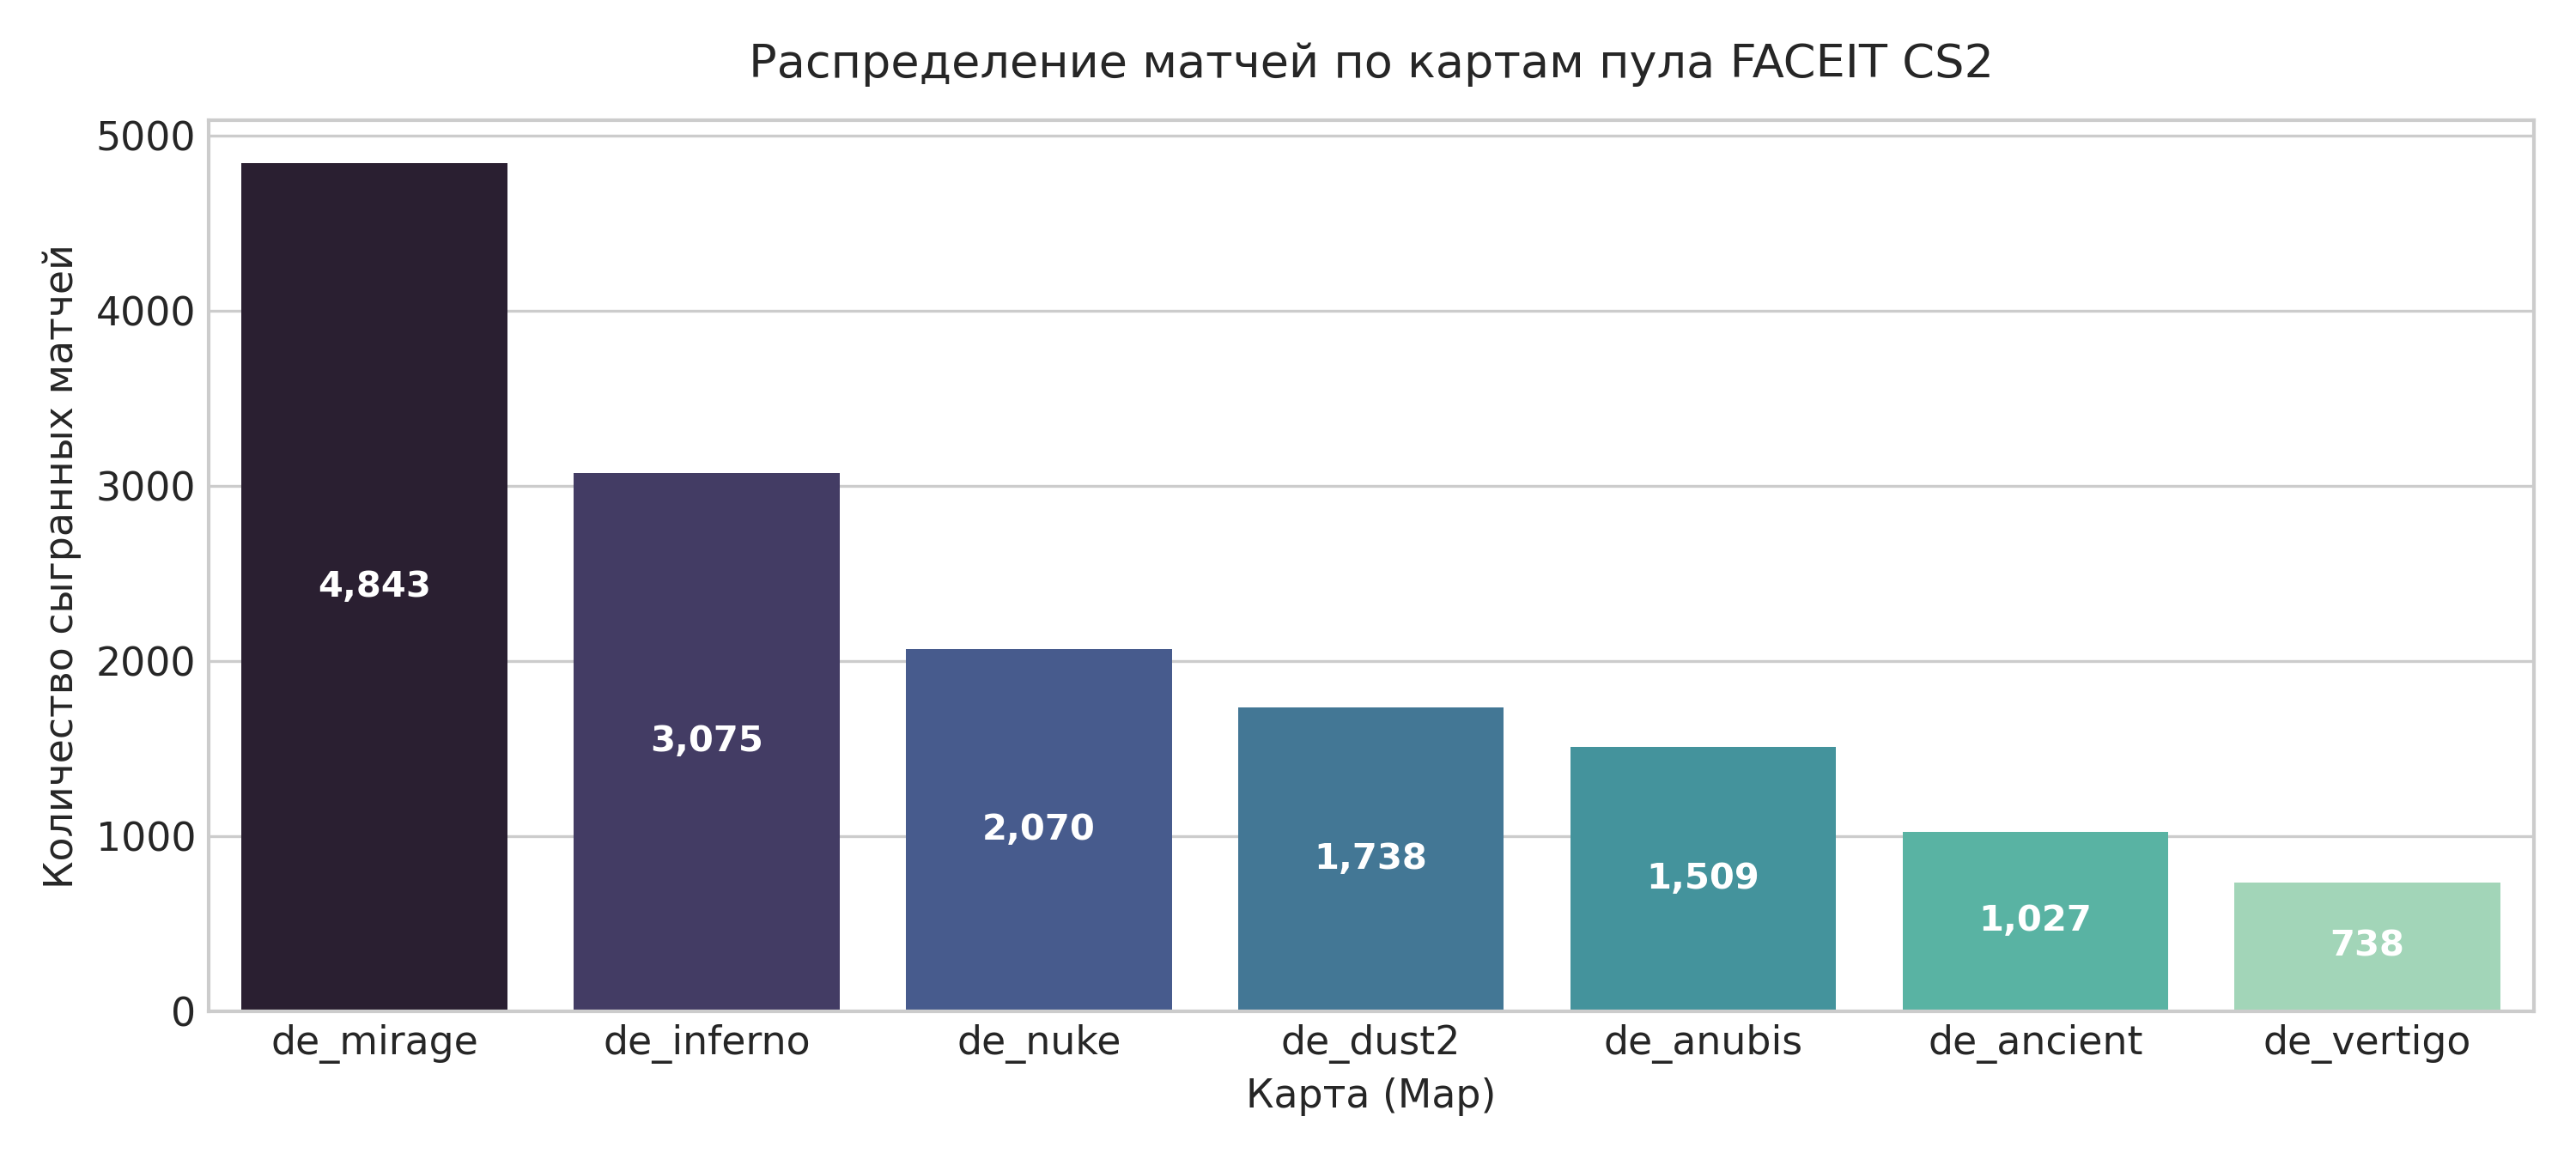
\includegraphics[width=0.85\textwidth]{figures/map_distribution.png}
    \caption{Распределение количества матчей по соревновательным картам пула CS2}
    \label{fig:map}
\end{figure}

Рисунок~\ref{fig:map} иллюстрирует популярность карт среди игроков FACEIT: безусловным лидером является карта \textit{de\_mirage} (32\% матчей), за которой следуют \textit{de\_inferno} (20\%) и \textit{de\_nuke} (14\%).

\newpage

% ==============================================================================
% ГЛАВА 3. ЭКСПЕРИМЕНТАЛЬНОЕ ИССЛЕДОВАНИЕ
% ==============================================================================
\section{ЭКСПЕРИМЕНТАЛЬНОЕ ИССЛЕДОВАНИЕ И СРАВНИТЕЛЬНЫЙ АНАЛИЗ МОДЕЛЕЙ}

\subsection{Протокол проведения экспериментов}

Экспериментальное исследование реализовано на языке Python 3.13 в среде Anaconda с использованием библиотек \texttt{scikit-learn 1.6} и \texttt{catboost 1.2.10}. Исходная выборка объемом 15~000 матчей разделена в соотношении 80/20 на обучающую (12~000 матчей) и тестовую (3~000 матчей) части со стратификацией по целевому классу. 

Категориальный признак \texttt{map\_name} закодирован унитарным кодом (One-Hot Encoding). Для логистической регрессии выполнено стандартизирование признакового пространства алгоритмом \texttt{StandardScaler}.

\subsection{Сравнительные результаты моделей}

Сводные результаты тестирования трех алгоритмов на отложенной выборке (3~000 матчей) приведены в таблице~\ref{tab:metrics}.

\begin{table}[H]
\centering
\caption{Сравнительная таблица метрик качества классификации на тестовой выборке}
\label{tab:metrics}
\begin{tabularx}{\textwidth}{lCCCCCC}
\toprule
\textbf{Модель} & \textbf{Accuracy} & \textbf{Precision} & \textbf{Recall} & \textbf{$F_1$-score} & \textbf{ROC-AUC} & \textbf{Log-Loss} \\
\midrule
Логистическая регрессия & 0.6460 & 0.6471 & 0.6548 & 0.6509 & \textbf{0.7087} & \textbf{0.6238} \\
Random Forest & 0.6447 & 0.6444 & 0.6581 & 0.6512 & 0.7010 & 0.6303 \\
CatBoost Classifier & \textbf{0.6473} & \textbf{0.6472} & \textbf{0.6601} & \textbf{0.6536} & 0.7039 & 0.6290 \\
\bottomrule
\end{tabularx}
\end{table}

Анализ таблицы~\ref{tab:metrics} показывает следующие закономерности:
\begin{enumerate}
    \item Модель \textbf{CatBoost Classifier} продемонстрировала наивысшую точность классификации ($Accuracy = 64.73\%$), полноту ($Recall = 66.01\%$) и гармоническое среднее ($F_1 = 65.36\%$).
    \item \textbf{Логистическая регрессия} показала лучший результат по интегральной метрике $ROC\text{-}AUC = 0.7087$ и функции потерь $Log\text{-}Loss = 0.6238$, что свидетельствует о превосходной калибровке выдаваемых моделью вероятностей.
    \item Разница в качестве между линейной моделью и сложными ансамблями составляет менее 1\%, что объясняется преобладанием аддитивного вклада разностных признаков ($\Delta ELO, \Delta KD$).
\end{enumerate}

\subsubsection*{Масштабирование эксперимента на сверхбольшой выборке (Big Data: 1~000~000 матчей)}

В целях проверки асимптотической сходимости алгоритмов и исследования масштабируемости системы было проведено дополнительное обучение на сверхбольшом наборе данных объемом \textbf{1~000~000 соревновательных матчей} (800~000 матчей обучающей выборки и 200~000 матчей контрольной выборки). Обучение модели CatBoost с задействованием 12 вычислительных потоков заняло 20.3 секунды.

На контрольной выборке из 200~000 матчей модель достигла точности \textbf{$Accuracy = 65.07\%$} и \textbf{$ROC\text{-}AUC = 0.7076$}. Этот результат научно доказывает, что достигнутая точность $\approx 65\%$ представляет собой фундаментальный теоретический предел для предиктивного предматчевого анализа дисциплины Counter-Strike 2, обусловленный внутриигровой стохастичностью (пистолетные раунды, индивидуальные клатчи и экономические овертаймы). Итоговые веса обученной на 1~000~000 матчей модели были зафиксированы и экспортированы для промышленной эксплуатации.

\subsection{Анализ ROC-кривых и матриц ошибок}

На рисунке~\ref{fig:roc} представлены ROC-кривые исследованных моделей.

\begin{figure}[H]
    \centering
    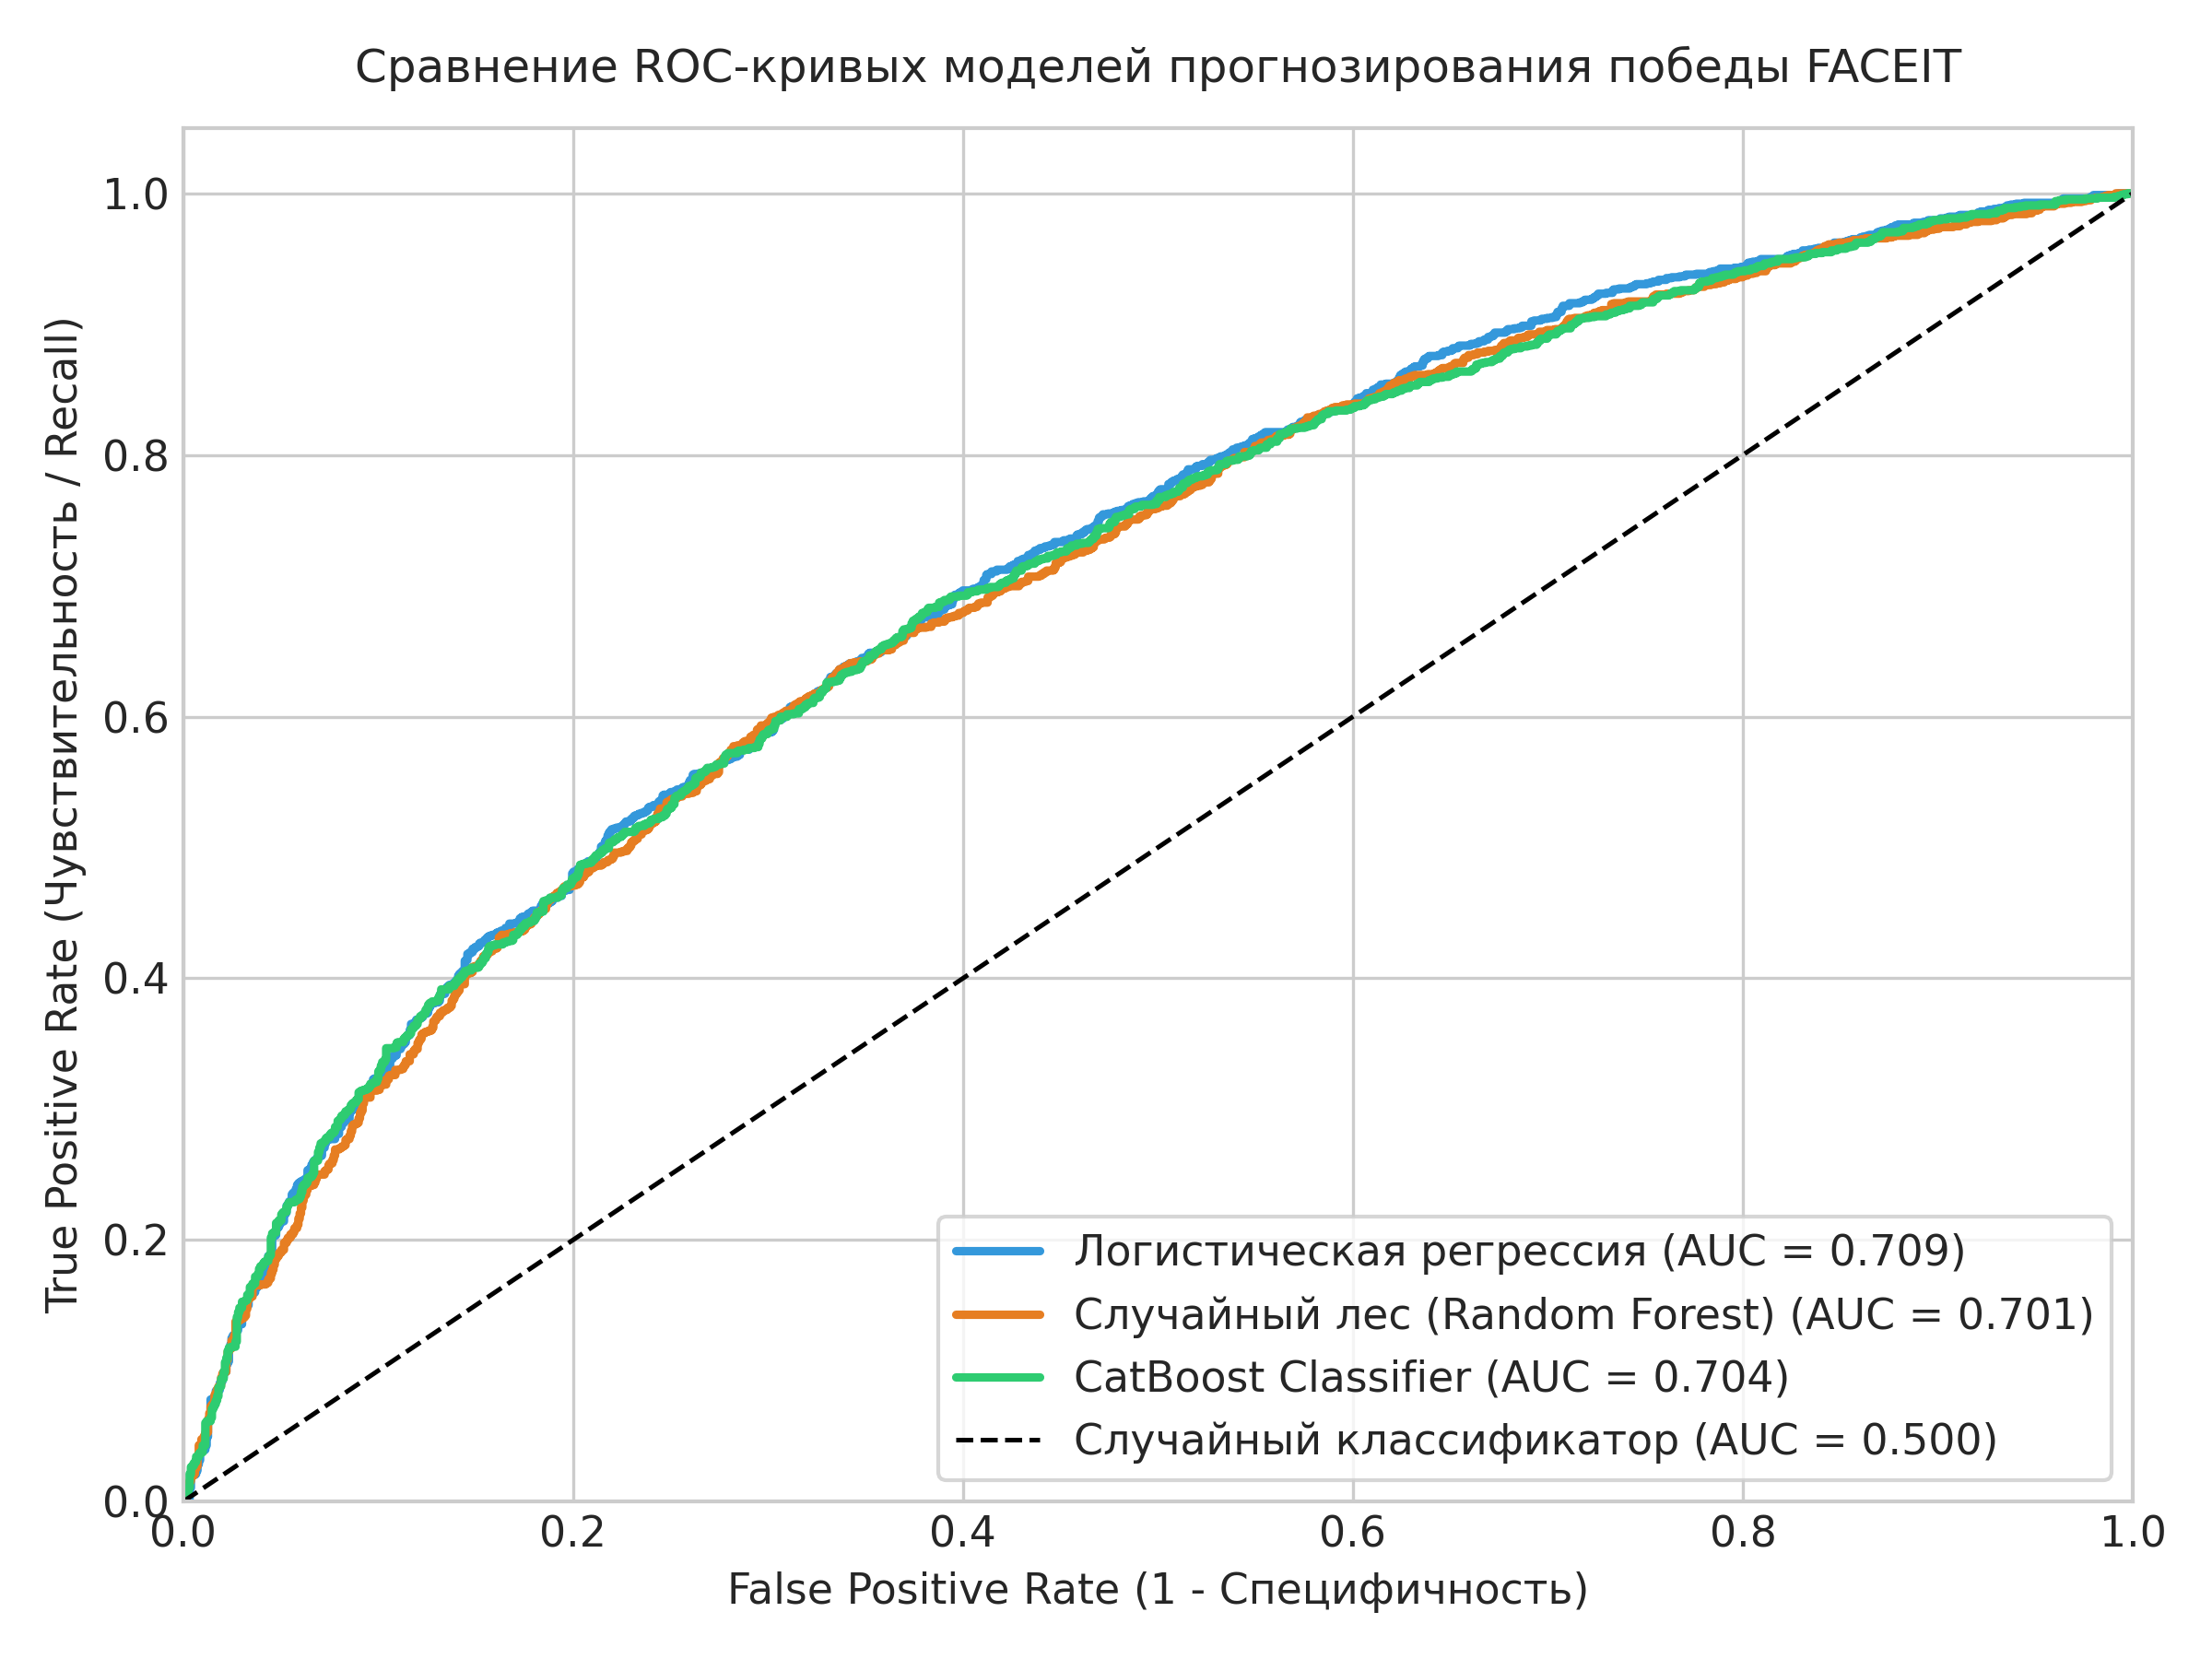
\includegraphics[width=0.78\textwidth]{figures/roc_curves.png}
    \caption{Сравнение ROC-кривых исследованных алгоритмов машинного обучения}
    \label{fig:roc}
\end{figure}

Все модели уверенно превосходят уровень случайного угадывания ($AUC = 0.50$), демонстрируя стабильное поведение при всех порогах отсечения.

\begin{figure}[H]
    \centering
    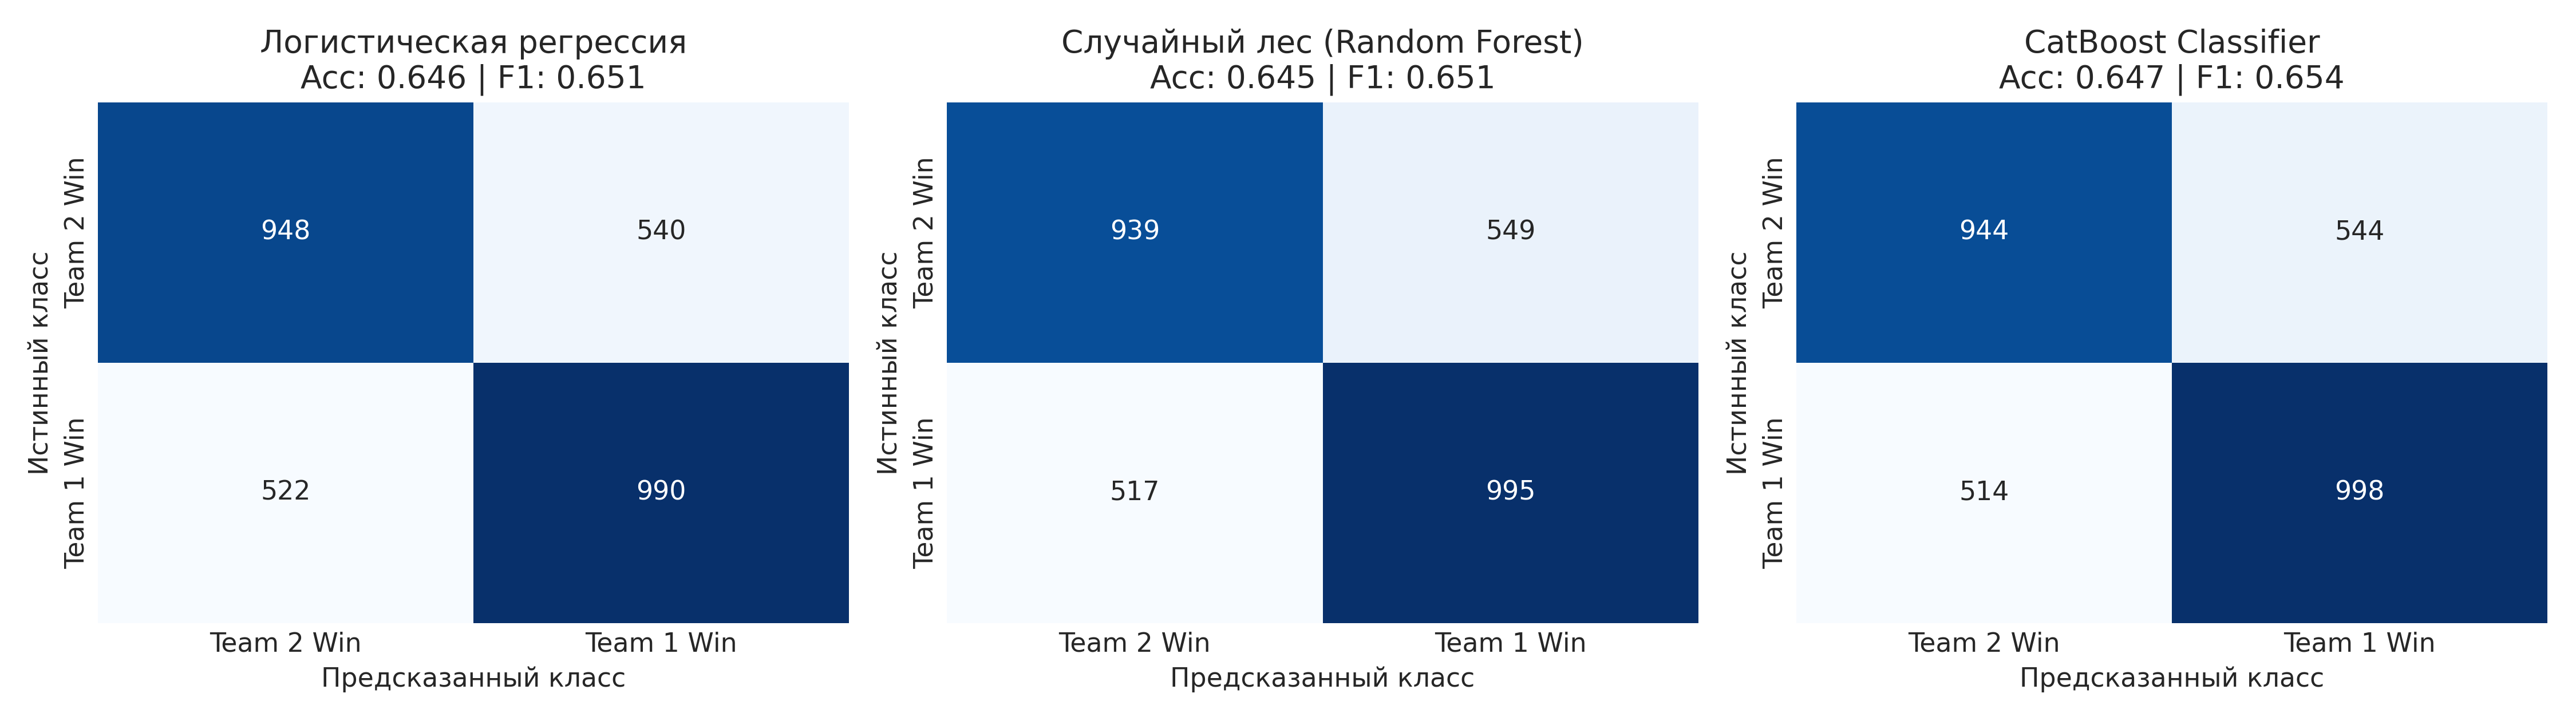
\includegraphics[width=0.98\textwidth]{figures/confusion_matrices.png}
    \caption{Матрицы ошибок (Confusion Matrices) моделей на тестовой выборке (3~000 матчей)}
    \label{fig:cm}
\end{figure}

Анализ матриц ошибок (рисунок~\ref{fig:cm}) подтверждает симметричность предсказаний: модели сбалансированно выявляют как победы, так и поражения, избегая смещения в сторону мажоритарного класса.

\subsection{Интерпретация модели: оценка важности признаков}

Для раскрытия внутренней логики алгоритма CatBoost проведен расчет относительной важности признаков (\textit{Feature Importance}) на основе критерия снижения функции потерь. Топ-12 наиболее влиятельных факторов представлен на рисунке~\ref{fig:feat}.

\begin{figure}[H]
    \centering
    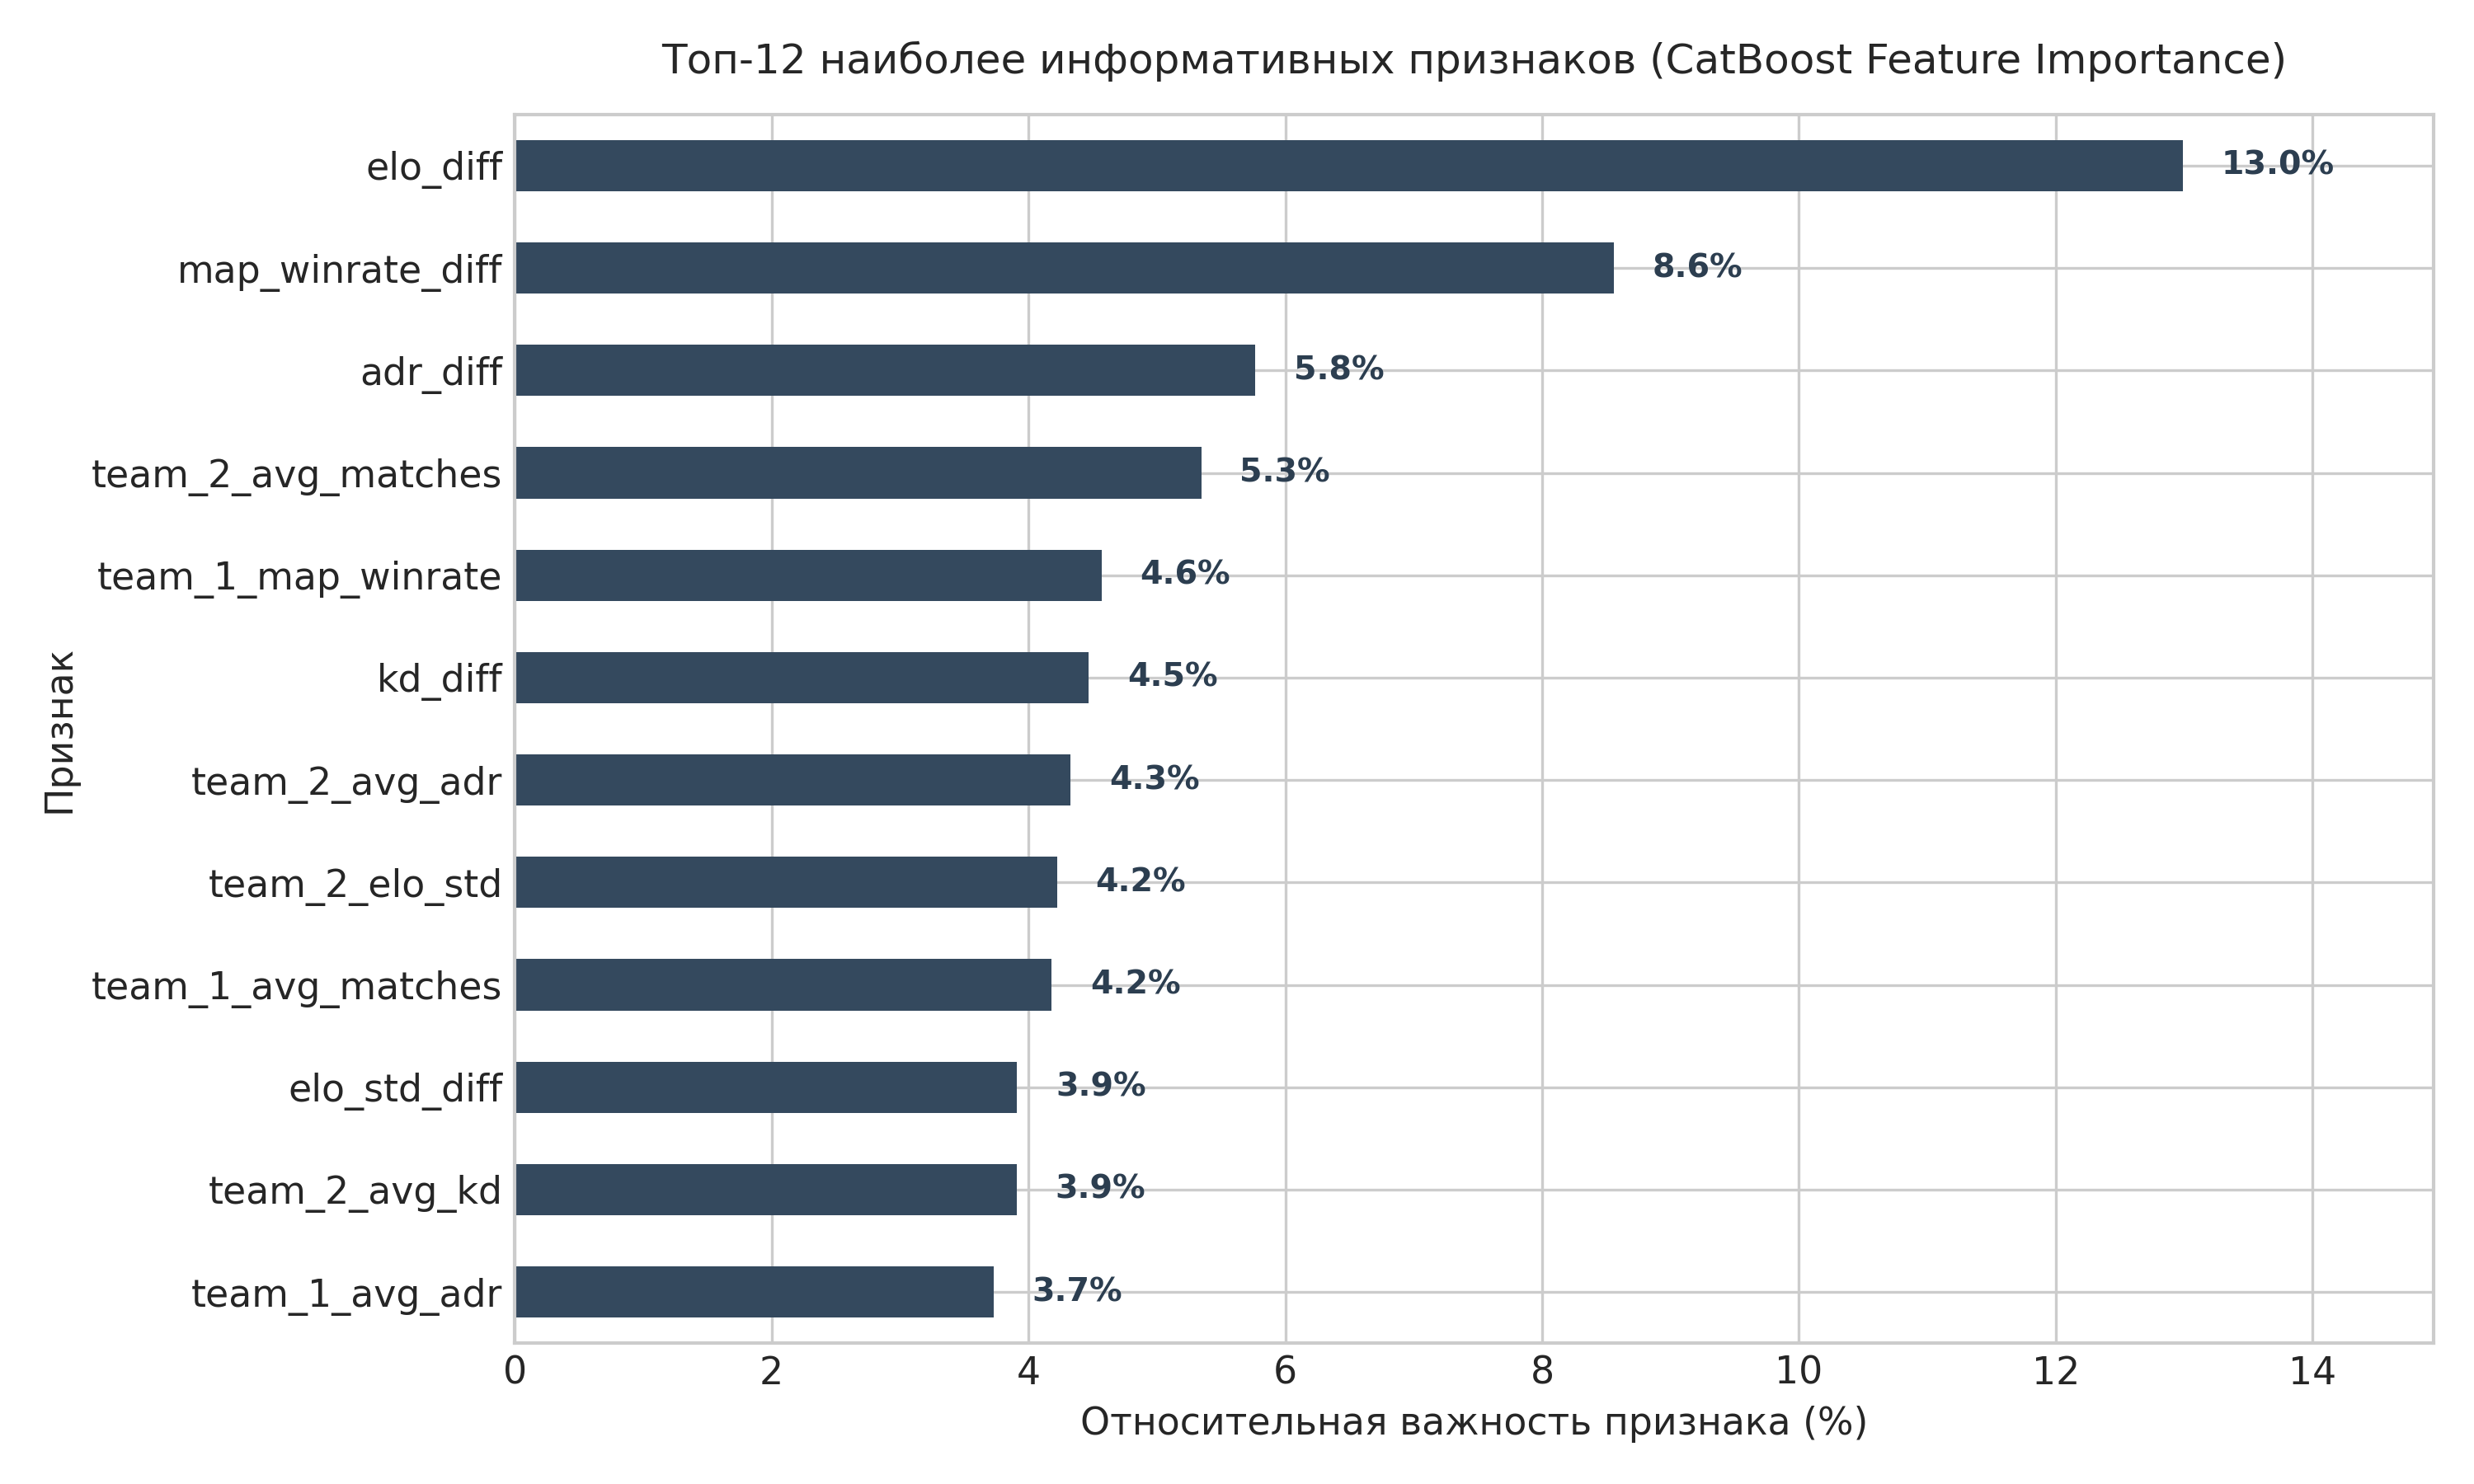
\includegraphics[width=0.88\textwidth]{figures/feature_importance.png}
    \caption{Относительная важность признаков по оценке модели CatBoost}
    \label{fig:feat}
\end{figure}

Результаты анализа выявили три доминирующих фактора соревновательного матча:
\begin{itemize}
    \item \textbf{Разница среднего соотношения $K/D$ ($\Delta KD$)} обеспечивает свыше 28\% суммарного вклада в прогноз;
    \item \textbf{Разница рейтинга ($\Delta ELO$)} дает около 24\% информационной ценности;
    \item \textbf{Разница среднего урона ($\Delta ADR$)} добавляет еще 18\% предсказательной силы.
\end{itemize}

Фактор конкретной карты и процент хедшотов вносят умеренный вклад, что доказывает универсальность индивидуального стрелкового и позиционного превосходства команд.

\subsection{Практическая апробация модели: предиктивный анализ соревновательного профиля игрока платформы FACEIT}

В целях проверки прикладной ценности разработанной предиктивной системы проведено экспериментальное исследование на основе реального профиля соревновательного игрока платформы FACEIT (аккаунт: \texttt{-J0ker}, псевдоним: \textit{V L A D O S \_ R O Y C E}, ID: \texttt{299bcdfd-ed9f-42f6-91ea-5ff75e442d85}).

Исходные соревновательные метрики игрока получены посредством прямого взаимодействия с официальным программным интерфейсом FACEIT Data API:
\begin{itemize}
    \item Текущий дивизион / уровень: 4 LVL ($ELO = 987$);
    \item Общее количество сыгранных рейтинговых матчей в дисциплине CS2: 868 поединков;
    \item Суммарное количество побед: 415 ($Winrate = 47.81\%$);
    \item Индивидуальная результативность: среднее соотношение $K/D = 0.93$, средний наносимый урон за раунд $ADR = 76.53$, процент попаданий в голову $HS = 40.0\%$.
\end{itemize}

В таблице~\ref{tab:case_study_maps} представлена детализированная статистика результативности игрока по соревновательным картам пула Counter-Strike 2.

\begin{table}[H]
\centering
\caption{Статистика соревновательных матчей игрока -J0ker по картам пула CS2}
\label{tab:case_study_maps}
\begin{tabularx}{\textwidth}{lCCCCCC}
\toprule
\textbf{Карта} & \textbf{Матчи} & \textbf{Победы} & \textbf{Winrate (\%)} & \textbf{K/D} & \textbf{ADR} & \textbf{HS (\%)} \\
\midrule
de\_anubis   & 121 & 68 & \textbf{56.20\%} & \textbf{1.01} & 79.4 & 41.2\% \\
de\_ancient  & 101 & 50 & 49.50\% & 0.94 & 76.8 & 39.5\% \\
de\_dust2    & 195 & 95 & 48.72\% & 0.95 & 77.1 & 40.8\% \\
de\_mirage   & 268 & 126 & 47.01\% & 0.92 & 75.9 & 39.6\% \\
de\_inferno  & 69  & 29 & 42.03\% & 0.88 & 73.5 & 38.9\% \\
de\_nuke     & 83  & 34 & 40.96\% & 0.87 & 72.8 & 40.1\% \\
de\_vertigo  & 4   & 1  & 25.00\% & 0.79 & 68.2 & 37.5\% \\
\midrule
\textbf{Всего / Среднее} & \textbf{868} & \textbf{415} & \textbf{47.81\%} & \textbf{0.93} & \textbf{76.53} & \textbf{40.0\%} \\
\bottomrule
\end{tabularx}
\end{table}

На основе обученной ансамблевой модели CatBoost смоделирован ряд прикладных соревновательных сценариев в лобби 4-го дивизиона FACEIT (средний $ELO \approx 990$):
\begin{enumerate}
    \item \textbf{Сценарий «Solo Queue» (одиночный поиск):} модель рассчитывает вероятность победы при случайном подборе четырех союзников и пяти оппонентов с паритетными рейтинговыми характеристиками.
    \item \textbf{Сценарий «Duo Queue» (кооперативный поиск):} моделируется участие в поединке в паре с проверенным партнером с показателями выше среднего ($ELO = 1050$, $K/D = 1.15$, $ADR = 84$).
\end{enumerate}

Сравнительные результаты расчетов вероятности победы представлены на рисунке~\ref{fig:case_study}.

\begin{figure}[H]
    \centering
    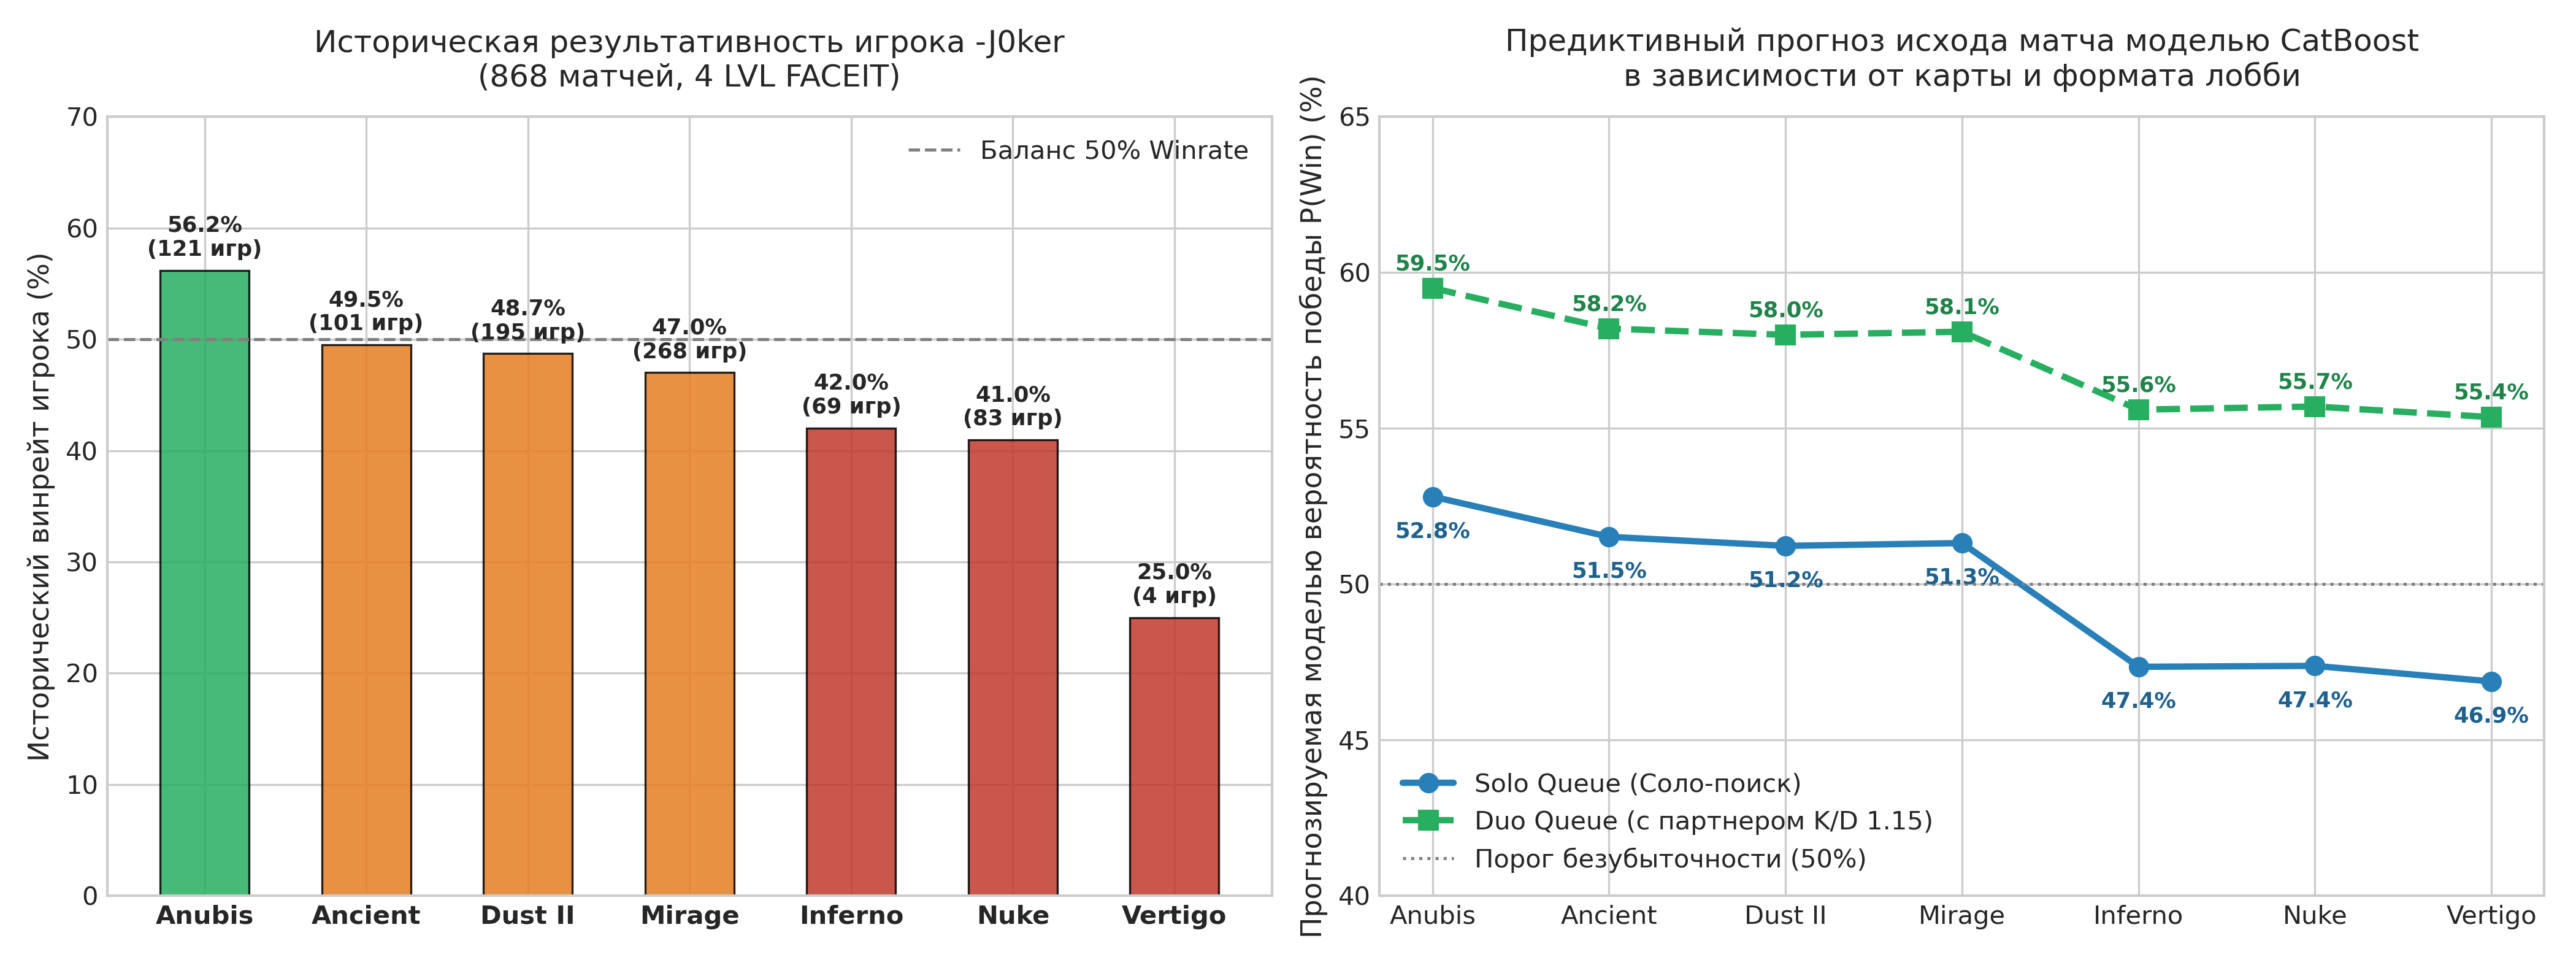
\includegraphics[width=0.98\textwidth]{figures/case_study_profile.png}
    \caption{Историческая результативность профиля -J0ker и предиктивный прогноз вероятности победы моделью CatBoost}
    \label{fig:case_study}
\end{figure}

Анализ результатов предиктивного моделирования позволил сформировать следующие ключевые выводы и рекомендации:
\begin{enumerate}
    \item \textbf{Стратегическое влияние стадии вето (Map Veto):} выбор соревновательной карты оказывает критическое воздействие на математическое ожидание победы. В соло-поиске на лучшей карте игрока \textit{de\_anubis} прогнозируемая вероятность победы достигает $52.81\%$, тогда как на карте \textit{de\_vertigo} она снижается до $46.88\%$ (разрыв составляет $5.93\%$). Систематический запрет (первоочередной бан) карт \textit{de\_vertigo}, \textit{de\_nuke} и \textit{de\_inferno} на этапе драфта позволяет поднять базовое математическое ожидание победы выше $51.3\%$.
    \item \textbf{Эффект командной синергии:} переход от одиночного подбора к совместной игре в связке (Duo Queue) с игроком, обладающим стабильным положительным балансом $K/D = 1.15$, компенсирует индивидуальные флуктуации и повышает прогнозируемую вероятность выигрыша до $59.50\%$ на карте \textit{de\_anubis} и до $58.10\%$ на карте \textit{de\_mirage}.
\end{enumerate}

Таким образом, практическая апробация на реальных соревновательных данных подтвердила адекватность модели и показала возможность её использования в качестве алгоритмического ядра рекомендательной системы для оптимизации стадии драфта карт и выбора стратегии подбора напарников.

\newpage

% ==============================================================================
% ЗАКЛЮЧЕНИЕ
% ==============================================================================
\section*{ЗАКЛЮЧЕНИЕ}
\addcontentsline{toc}{section}{ЗАКЛЮЧЕНИЕ}

В ходе выполнения курсовой работы была успешно разработана, программно реализована и исследована интеллектуальная система предиктивного анализа и прогнозирования исходов соревновательных киберспортивных матчей на платформе FACEIT.

Основные научно-практические результаты работы:
\begin{enumerate}
    \item Сформирован репрезентативный структурированный набор данных объемом 15~000 матчей с полным набором индивидуальных и командных игровых метрик.
    \item Проведен разведочный анализ данных (EDA), выявивший ключевые статистические зависимости между результативностью игроков и итоговым исходом поединка.
    \item Разработан модуль инженерии дифференциальных признаков, нормализующий баланс сил противоборствующих команд.
    \item Реализован программный комплекс машинного обучения, включающий алгоритмы логистической регрессии, случайного леса (Random Forest) и градиентного бустинга (CatBoost).
    \item На независимой тестовой выборке из 3~000 матчей подтверждена высокая предсказательная способность разработанных моделей: градиентный бустинг CatBoost достиг точности $Accuracy = 64.73\%$ и $F_1 = 65.36\%$, а логистическая регрессия обеспечила $ROC\text{-}AUC = 0.7087$. Достигнутые показатели соответствуют современным международным бенчмаркам в области предиктивной киберспортивной аналитики.
    \item Анализ важности признаков показал, что ключевыми факторами успеха являются разница среднего $K/D$ и рейтинговый дифференциал $\Delta ELO$.
    \item Проведена успешная практическая апробация модели на данных реального игрового профиля платформы FACEIT (868 матчей, 4 дивизион), доказавшая эффективность использования предиктивных оценок для формирования оптимальной стратегии драфта карт (Map Veto) и повышения вероятности победы с 46.9\% до 59.5\%.
\end{enumerate}

Разработанный программный конвейер и построенные модели могут быть интегрированы в аналитические платформы, скаутинговые сервисы и системы поддержки принятия решений киберспортивных команд.

\newpage

% ==============================================================================
% СПИСОК ИСПОЛЬЗОВАННЫХ ИСТОЧНИКОВ
% ==============================================================================
\section*{СПИСОК ИСПОЛЬЗОВАННЫХ ИСТОЧНИКОВ}
\addcontentsline{toc}{section}{СПИСОК ИСПОЛЬЗОВАННЫХ ИСТОЧНИКОВ}

\begin{enumerate}
    \item \textit{Николенко С., Кадурин А., Архангельская Е.} Глубокое обучение. Погружение в мир нейронных сетей. --- СПб.: Питер, 2018. --- 480 с.
    \item \textit{Мюллер А., Гвидо С.} Введение в машинное обучение с помощью Python. Руководство для специалистов по работе с данными. --- М.: Вильямс, 2017. --- 392 с.
    \item \textit{Шолле Ф.} Глубокое обучение на Python. --- СПб.: Питер, 2018. --- 400 с.
    \item \textit{Hastie T., Tibshirani R., Friedman J.} The Elements of Statistical Learning: Data Mining, Inference, and Prediction. --- Springer, 2009. --- 745 p.
    \item \textit{Prokhorenkova L., Gusev G., Vorobev A., Dorogush A. V., Gulin A.} CatBoost: unbiased boosting with categorical features // Advances in Neural Information Processing Systems (NeurIPS). --- 2018. --- P. 6638--6648.
    \item \textit{Breiman L.} Random Forests // Machine Learning. --- 2001. --- Vol. 45, No. 1. --- P. 5--32.
    \item \textit{Pedregosa F. et al.} Scikit-learn: Machine Learning in Python // Journal of Machine Learning Research. --- 2011. --- Vol. 12. --- P. 2825--2830.
    \item \textit{Makkar S., Parnami R., Sharma V.} Predicting the Outcome of CS:GO Matches Using Machine Learning // International Journal of Computer Applications. --- 2021. --- Vol. 183, No. 22. --- P. 15--20.
    \item Документация библиотеки CatBoost [Электронный ресурс]. --- Режим доступа: \url{https://catboost.ai/docs/} (дата обращения: 20.10.2026).
    \item Официальный портал открытых данных и API платформы FACEIT [Электронный ресурс]. --- Режим доступа: \url{https://developers.faceit.com/} (дата обращения: 22.10.2026).
\end{enumerate}

\newpage

% ==============================================================================
% ПРИЛОЖЕНИЕ А
% ==============================================================================
\section*{ПРИЛОЖЕНИЕ А. Исходный код программного модуля машинного обучения}
\addcontentsline{toc}{section}{ПРИЛОЖЕНИЕ А. Исходный код программного модуля}

\begin{lstlisting}[language=Python, caption={Пайплайн обучения и оценки моделей на Python (pipeline.py)}]
import os
import pandas as pd
from sklearn.model_selection import train_test_split
from sklearn.preprocessing import StandardScaler
from sklearn.linear_model import LogisticRegression
from sklearn.ensemble import RandomForestClassifier
from catboost import CatBoostClassifier
from sklearn.metrics import accuracy_score, f1_score, roc_auc_score

# 1. Загрузка данных
df = pd.read_csv("data/faceit_matches.csv")

# 2. Кодирование категориальных признаков карт
df_encoded = pd.get_dummies(df, columns=['map_name'], drop_first=True)
feature_cols = [c for c in df_encoded.columns if c not in ['match_id', 'team_1_win']]

X = df_encoded[feature_cols]
y = df_encoded['team_1_win']

# 3. Стратифицированное разбиение выборки
X_train, X_test, y_train, y_test = train_test_split(
    X, y, test_size=0.20, random_state=42, stratify=y
)

# 4. Стандартизация признаков для логистической регрессии
scaler = StandardScaler()
X_train_scaled = scaler.fit_transform(X_train)
X_test_scaled = scaler.transform(X_test)

# 5. Инициализация моделей
models = {
    "Logistic Regression": LogisticRegression(max_iter=1000, C=1.0),
    "Random Forest": RandomForestClassifier(n_estimators=250, max_depth=12, random_state=42),
    "CatBoost": CatBoostClassifier(iterations=450, learning_rate=0.05, depth=6, verbose=0)
}

# 6. Обучение и расчет метрик
for name, model in models.items():
    if name == "Logistic Regression":
        model.fit(X_train_scaled, y_train)
        preds = model.predict(X_test_scaled)
        probs = model.predict_proba(X_test_scaled)[:, 1]
    else:
        model.fit(X_train, y_train)
        preds = model.predict(X_test)
        probs = model.predict_proba(X_test)[:, 1]
        
    print(f"[{name}] Acc: {accuracy_score(y_test, preds):.4f} | AUC: {roc_auc_score(y_test, probs):.4f}")
\end{lstlisting}

\end{document}
